\documentclass[10pt,aspectratio=169]{beamer}

% Theme and Color Setup
\usetheme{Madrid}
\usecolortheme{beaver}

% Packages
\usepackage[utf8]{inputenc}
\usepackage{graphicx}
\usepackage{amsmath,amssymb}
\usepackage{booktabs}
\usepackage{array}
\usepackage{tikz}
\usetikzlibrary{shapes.geometric, arrows, positioning, fit, calc, shadows, backgrounds}
\usepackage{listings}
\usepackage{xcolor}

% Custom Colors
\definecolor{primaryBlue}{RGB}{24, 76, 120}
\definecolor{accentNavy}{RGB}{15, 32, 67}
\definecolor{bgGray}{RGB}{248, 249, 250}
\definecolor{darkText}{RGB}{33, 37, 41}

\setbeamercolor{palette primary}{bg=primaryBlue,fg=white}
\setbeamercolor{palette secondary}{bg=accentNavy,fg=white}
\setbeamercolor{palette tertiary}{bg=primaryBlue!80,fg=white}
\setbeamercolor{titlelike}{parent=palette primary}
\setbeamercolor{structure}{fg=primaryBlue}

% Code Listing Setup
\lstdefinestyle{mystyle}{
    backgroundcolor=\color{black!5},   
    commentstyle=\color{green!60!black},
    keywordstyle=\color{blue!80!black},
    numberstyle=\tiny\color{gray},
    stringstyle=\color{purple},
    basicstyle=\ttfamily\scriptsize,
    breakatwhitespace=false,         
    breaklines=true,                 
    captionpos=b,                    
    keepspaces=true,                 
    numbers=left,                    
    numbersep=5pt,                  
    showspaces=false,                
    showstringspaces=false,
    showtabs=false,                  
    tabsize=2
}
\lstset{style=mystyle}

% --------------------------------------------------
% TITLE SLIDE INFO
% --------------------------------------------------
\title[LegalAssist - Final Evaluation]{LegalAssist}
\subtitle{Smart AI Legal Assistant and Advocate Appointment \& Case Management System\\{\small Final Evaluation Presentation}}

\author[ABHISHEK ANAND]{%
  \textbf{Name:} ABHISHEK ANAND \\
  \textbf{KTU ID:} KTE25MCA-2002 \\
  \textbf{Guide:} Prof. REENA MURALI
}

\institute[RIT Kottayam]{
  Department of Computer Applications\\
  Rajiv Gandhi Institute of Technology (RIT), Kottayam\\
  Government Engineering College, Kerala - 686501
}

\date{2026}

\begin{document}

% Slide 1: Title
\begin{frame}
  \titlepage
\end{frame}

% Slide 2: Introduction
\begin{frame}{Introduction}
  \begin{itemize}
    \setlength{\itemsep}{10pt}
    \item \textbf{LegalAssist} is a full-stack web application designed to bridge the gap between citizens seeking legal aid and verified legal advocates.
    \item Connects three key user roles: \textbf{Clients / Citizens}, \textbf{Advocates}, and \textbf{System Administrators}.
    \item Enables real-time advocate discovery, transparent consultation appointment scheduling, and automated weekly schedule management.
    \item Integrates structured \textbf{Case Lifecycle Tracking} with visual stage updates from initial consultation to final judgment.
    \item Features an \textbf{AI-Powered Legal Assistant} for 24/7 layman-friendly guidance on Indian legal codes (IPC, BNS, CrPC, BNSS, CPC) alongside an emergency \textbf{SOS Alert System}.
  \end{itemize}
\end{frame}

% Slide 3: Requirement Analysis
\begin{frame}{Requirement Analysis}
  \begin{columns}[T]
    \begin{column}{0.48\textwidth}
      \begin{block}{\textbf{Functional Requirements}}
        \begin{itemize}
          \item Multi-role user registration and login.
          \item Advocate Bar Council document verification workflow.
          \item Real-time weekly slot booking \& double-booking prevention.
          \item Case stage timeline \& document management.
          \item AI Legal Assistant chatbot integration.
          \item Emergency SOS alert broadcasting center.
        \end{itemize}
      \end{block}
    \end{column}
    
    \begin{column}{0.48\textwidth}
      \begin{block}{\textbf{Non-Functional Requirements}}
        \begin{itemize}
          \item \textbf{Responsiveness}: Mobile \& desktop friendly UI.
          \item \textbf{Security}: Password hashing with bcrypt.
          \item \textbf{Reliability}: Dual-engine persistence (Local JSON + MongoDB Atlas).
          \item \textbf{Performance}: Sub-second API response times and instant server listener initialization.
          \item \textbf{Usability}: Intuitive glassmorphism interface.
        \end{itemize}
      \end{block}
    \end{column}
  \end{columns}
\end{frame}

% Slide 4: Problem Statement
\begin{frame}{Problem Statement}
  \begin{itemize}
    \setlength{\itemsep}{12pt}
    \item \textbf{Fragmented Legal Aid Discovery}: Finding verified legal professionals relies heavily on word-of-mouth with no central verification audit.
    \item \textbf{Scheduling Friction}: Manual phone calls and offline coordination lead to double-booked appointments and missed consultations.
    \item \textbf{Opaque Case Tracking}: Clients lack visibility into case stage progression, court hearing dates, and document updates.
    \item \textbf{Complex Legal Terminology}: Citizens struggle to understand basic statutory rights, legal sections, and procedures during emergencies.
    \item \textbf{Proposed Solution}: \textbf{LegalAssist} unifies advocate verification, automated slot booking, transparent case tracking, AI aid, and emergency SOS into a single integrated digital platform.
  \end{itemize}
\end{frame}

% Slide 5: Objectives
\begin{frame}{Objectives}
  \begin{itemize}
    \setlength{\itemsep}{10pt}
    \item Build a secure, role-based platform for Clients, Advocates, and Admins.
    \item Implement an Admin audit workflow for Advocate credential verification before public directory listing.
    \item Develop an automated schedule engine allowing Advocates to define weekly availability and prevent double-booking.
    \item Provide visual Case Stage Tracking (Consultation $\rightarrow$ Hearing $\rightarrow$ Judgment $\rightarrow$ Closure) with document attachments.
    \item Deploy an AI Legal Chatbot backed by an offline Indian Legal Knowledge Base (IPC, BNS, CrPC, BNSS) with Cloud AI fallback.
    \item Provide a one-click Emergency SOS Alert system for instant citizen safety assistance.
  \end{itemize}
\end{frame}

% Slide 6: Scope and Relevance
\begin{frame}{Scope and Relevance}
  \begin{columns}[T]
    \begin{column}{0.48\textwidth}
      \begin{block}{\textbf{Project Scope}}
        \begin{itemize}
          \item Multi-role user authentication \& profile management.
          \item Advocate search, filtering by specialization, fee, rating, and location.
          \item Interactive appointment booking and status updates.
          \item Complete case lifecycle management.
          \item AI legal assistant & emergency SOS alert modal.
        \end{itemize}
      \end{block}
    \end{column}
    
    \begin{column}{0.48\textwidth}
      \begin{block}{\textbf{Societal & Technical Relevance}}
        \begin{itemize}
          \item Democratizes access to verified legal professionals.
          \item Eliminates consultation scheduling conflicts.
          \item Provides 24/7 legal literacy and emergency aid for citizens.
          \item Zero-downtime hybrid database architecture ensures local accessibility even during cloud outages.
        \end{itemize}
      \end{block}
    \end{column}
  \end{columns}
\end{frame}

% Slide 7: Development Methodology - Process
\begin{frame}{Development Methodology -- Process}
  \begin{itemize}
    \setlength{\itemsep}{10pt}
    \item \textbf{Agile / Incremental SDLC}: Development was executed in iterative modular phases to ensure continuous testing and refinement.
    \item \textbf{Pipeline Stages}:
      \begin{center}
        \small
        Requirement Analysis $\rightarrow$ System Architecture Design $\rightarrow$ Module Development $\rightarrow$ System Integration $\rightarrow$ Empirical Verification \& Testing
      \end{center}
    \item \textbf{Version Control}: Git source control maintained on GitHub (`abhishekanandgit/mini-project`) with clear commit milestones.
    \item \textbf{Build Validation}: Continuous automated syntax and bundling validation (`vite build` \& `node -c`).
  \end{itemize}
\end{frame}

% Slide 8: Development Methodology - Modules
\begin{frame}{Development Methodology -- Modules}
  \begin{enumerate}
    \setlength{\itemsep}{8pt}
    \item \textbf{Authentication \& Profile Module}: Role-based registration, login, profile editing, and document upload.
    \item \textbf{Advocate Verification Module}: Admin review interface for Bar Council credentials and approval/rejection workflows.
    \item \textbf{Availability \& Scheduling Engine}: Advocate weekly slot configuration and client real-time slot selection.
    \item \textbf{Case Management Module}: Stage timeline tracking, case note logs, and document repository.
    \item \textbf{AI Legal Assistant Module}: Indian Legal Knowledge Base query engine and Gemini API service.
    \item \textbf{Emergency SOS Module}: SOS alert trigger broadcast and resolution center.
    \item \textbf{Data & Persistence Module}: Dual-engine storage (`db.js`) supporting local JSON and MongoDB Atlas sync.
  \end{enumerate}
\end{frame}

% Slide 9: Development Methodology - Testing
\begin{frame}{Development Methodology -- Testing}
  \begin{itemize}
    \setlength{\itemsep}{10pt}
    \item \textbf{Authentication & Authorization Testing}: Verified role protection and access control across client, advocate, and admin routes.
    \item \textbf{Concurrency & Slot Validation}: Enforced double-booking prevention under simultaneous booking requests.
    \item \textbf{Hybrid DB Fallback Testing}: Verified zero-downtime local JSON database fallback during cloud DNS/network timeouts.
    \item \textbf{AI Knowledge Base Testing}: Checked legal query resolution across IPC, BNS, CrPC, and Constitutional FAQ modules.
    \item \textbf{End-to-End Cross-Browser Testing}: Validated responsive UI rendering across mobile, tablet, and desktop views.
  \end{itemize}
\end{frame}

% Slide 10: System Architecture
\begin{frame}{System Architecture}
  \begin{center}
    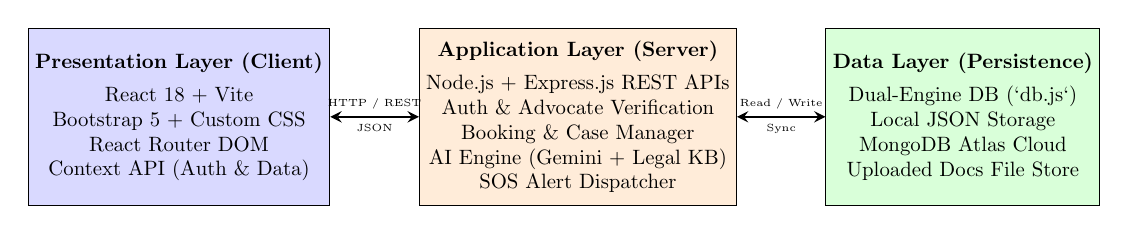
\begin{tikzpicture}[node distance=1.2cm, auto, >=stealth, scale=0.75, transform shape]
      % Presentation Layer
      \node [draw, rectangle, fill=blue!15, minimum width=3.8cm, minimum height=3cm, align=center] (client) {
        \textbf{Presentation Layer (Client)}\\[4pt]
        React 18 + Vite\\
        Bootstrap 5 + Custom CSS\\
        React Router DOM\\
        Context API (Auth \& Data)
      };
      
      % Application Layer
      \node [draw, rectangle, fill=orange!15, minimum width=4.5cm, minimum height=3cm, right=1.5cm of client, align=center] (server) {
        \textbf{Application Layer (Server)}\\[4pt]
        Node.js + Express.js REST APIs\\
        Auth \& Advocate Verification\\
        Booking \& Case Manager\\
        AI Engine (Gemini + Legal KB)\\
        SOS Alert Dispatcher
      };
      
      % Data Layer
      \node [draw, rectangle, fill=green!15, minimum width=3.8cm, minimum height=3cm, right=1.5cm of server, align=center] (data) {
        \textbf{Data Layer (Persistence)}\\[4pt]
        Dual-Engine DB (`db.js`)\\
        Local JSON Storage\\
        MongoDB Atlas Cloud\\
        Uploaded Docs File Store
      };
      
      % Arrows
      \draw [<->, thick] (client) -- node [above, font=\tiny] {HTTP / REST} node [below, font=\tiny] {JSON} (server);
      \draw [<->, thick] (server) -- node [above, font=\tiny] {Read / Write} node [below, font=\tiny] {Sync} (data);
    \end{tikzpicture}
  \end{center}
\end{frame}

% Slide 11: System Workflow
\begin{frame}{System Workflow}
  \begin{center}
    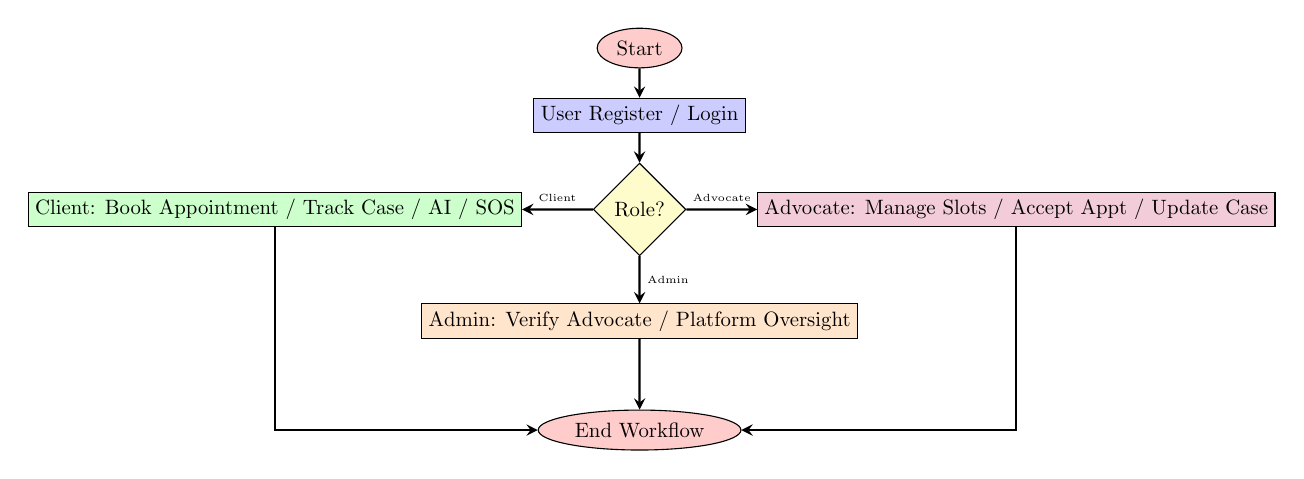
\begin{tikzpicture}[node distance=0.9cm, auto, >=stealth, scale=0.75, transform shape]
      \node [draw, ellipse, fill=red!20] (start) {Start};
      \node [draw, rectangle, fill=blue!20, below=0.5cm of start] (auth) {User Register / Login};
      \node [draw, diamond, fill=yellow!20, below=0.5cm of auth] (role) {Role?};
      
      \node [draw, rectangle, fill=green!20, left=1.2cm of role] (client) {Client: Book Appointment / Track Case / AI / SOS};
      \node [draw, rectangle, fill=purple!20, right=1.2cm of role] (adv) {Advocate: Manage Slots / Accept Appt / Update Case};
      \node [draw, rectangle, fill=orange!20, below=0.8cm of role] (admin) {Admin: Verify Advocate / Platform Oversight};
      
      \node [draw, ellipse, fill=red!20, below=1.2cm of admin] (end) {End Workflow};
      
      \draw [->, thick] (start) -- (auth);
      \draw [->, thick] (auth) -- (role);
      \draw [->, thick] (role) -- node [above, font=\tiny] {Client} (client);
      \draw [->, thick] (role) -- node [above, font=\tiny] {Advocate} (adv);
      \draw [->, thick] (role) -- node [right, font=\tiny] {Admin} (admin);
      \draw [->, thick] (client) |- (end);
      \draw [->, thick] (adv) |- (end);
      \draw [->, thick] (admin) -- (end);
    \end{tikzpicture}
  \end{center}
\end{frame}

% Slide 12: Implementation Details - Frontend
\begin{frame}{Implementation Details -- Frontend}
  \begin{itemize}
    \setlength{\itemsep}{10pt}
    \item \textbf{Framework}: Built with \textbf{React 18} and \textbf{Vite} for fast HMR and optimized production bundles.
    \item \textbf{State Management}: React Context API (`AuthContext`, `DataContext`) for global state, user session persistence, and real-time synchronization across views.
    \item \textbf{Styling}: Bootstrap 5 paired with custom CSS glassmorphism styling, clean typography, and interactive micro-animations.
    \item \textbf{Dynamic Rendering}: Responsive templates for Case Stage Timelines, Advocate Schedules, AI Chatbot modal, and Emergency SOS dialogs.
  \end{itemize}
\end{frame}

% Slide 13: Implementation Details - Backend and AI
\begin{frame}{Implementation Details -- Backend \& AI}
  \begin{itemize}
    \setlength{\itemsep}{10pt}
    \item \textbf{Server Infrastructure}: Engineered with \textbf{Node.js} and \textbf{Express.js} exposing modular REST API endpoints (`/api/auth`, `/api/advocates`, `/api/appointments`, `/api/cases`, `/api/sos`, `/api/ai/chat`).
    \item \textbf{AI Legal Engine}: Integrated legal query processing using an extensive **Indian Legal Knowledge Base** covering:
      \begin{itemize}
        \item Indian Penal Code (IPC) \& Bharatiya Nyaya Sanhita (BNS)
        \item Code of Criminal Procedure (CrPC) \& BNSS
        \item Code of Civil Procedure (CPC), Fundamental Rights \& Legal FAQs
      \end{itemize}
    \item \textbf{Cloud AI Fallback}: Seamless fallback between Google Gemini API and local knowledge retrieval.
  \end{itemize}
\end{frame}

% Slide 14: Implementation Details - Database & Security
\begin{frame}{Implementation Details -- Database \& Security}
  \begin{itemize}
    \setlength{\itemsep}{10pt}
    \item \textbf{Dual-Engine Database (`db.js`)}:
      \begin{itemize}
        \item Primary cloud persistence via \textbf{MongoDB Atlas}.
        \item Automatic, transparent fallback to local persistent JSON storage (`legalassist_db.json`) during cloud network timeouts.
      \end{itemize}
    \item \textbf{Security Practices}:
      \begin{itemize}
        \item Password protection using `bcrypt` hashing.
        \item Strict input validation and sanitize checks on registration & booking endpoints.
        \item Double-booking collision checks on time slots.
      \end{itemize}
    \item \textbf{Vite Proxy Error Handler}: Graceful handling of backend cold starts with HTTP 503 fallback responses.
  \end{itemize}
\end{frame}

% Slide 15: Results - Authentication & Registration
\begin{frame}{Results -- Authentication \& Registration}
  \begin{block}{\textbf{User Onboarding \& Role Selection}}
    \begin{itemize}
      \item Clean unified portal for Client, Advocate, and Admin login and registration.
      \item Advocate registration captures Bar Council Enrollment ID, legal specialization, experience years, consultation fees, and qualification documents.
      \item Enforces email uniqueness and secure credential hashing.
    \end{itemize}
  \end{block}
  \begin{center}
    \small \textit{[Features Client \& Advocate Signup with Bar ID \& Document Verification Submission]}
  \end{center}
\end{frame}

% Slide 16: Results - User & Advocate Dashboards
\begin{frame}{Results -- User \& Advocate Dashboards}
  \begin{columns}[T]
    \begin{column}{0.48\textwidth}
      \begin{block}{\textbf{User Dashboard}}
        \begin{itemize}
          \item Active appointment status.
          \item Interactive case stage tracking.
          \item One-click SOS trigger & review submission.
        \end{itemize}
      \end{block}
    \end{column}

    \begin{column}{0.48\textwidth}
      \begin{block}{\textbf{Advocate Dashboard}}
        \begin{itemize}
          \item Weekly slot availability editor.
          \item Appointment approval/rejection with reason grounds.
          \item Case stage progression & document management.
        \end{itemize}
      \end{block}
    \end{column}
  \end{columns}
\end{frame}

% Slide 17: Results - Advocate Directory & Booking
\begin{frame}{Results -- Advocate Directory \& Booking}
  \begin{block}{\textbf{Advocate Search \& Real-Time Appointment Booking}}
    \begin{itemize}
      \item **Search & Filter**: Search advocates by name, Bar ID, specialization (Criminal, Civil, Corporate, Family, Constitutional), location, and fee structure.
      \item **Real-Time Booking**: Select date and available time slots dynamically derived from the advocate's configured weekly schedule.
      \item **Conflict Resolution**: Prevents overlapping bookings for identical advocate time slots.
    \end{itemize}
  \end{block}
\end{frame}

% Slide 18: Results - Case Stage Timeline
\begin{frame}{Results -- Case Stage Timeline}
  \begin{block}{\textbf{Structured Case Lifecycle Management}}
    \begin{itemize}
      \item Visual step timeline detailing current case phase:
        \begin{center}
          \small \textbf{Consultation} $\rightarrow$ \textbf{Investigation} $\rightarrow$ \textbf{Hearing / Trial} $\rightarrow$ \textbf{Judgment} $\rightarrow$ \textbf{Case Closure}
        \end{center}
      \item Advocate can update active stage, attach stage notes, and upload relevant legal filings or evidence documents.
      \item Client gains full transparency into upcoming hearing dates and stage updates.
    \end{itemize}
  \end{block}
\end{frame}

% Slide 19: Results - AI Legal Assistant & Emergency SOS
\begin{frame}{Results -- AI Legal Assistant \& Emergency SOS}
  \begin{columns}[T]
    \begin{column}{0.48\textwidth}
      \begin{block}{\textbf{AI Legal Assistant}}
        \begin{itemize}
          \item 24/7 conversational assistant for legal queries.
          \item Explains legal sections, rights, and court procedures in plain layman terms.
          \item Powered by local Indian Legal KB with cloud Gemini fallback.
        \end{itemize}
      \end{block}
    \end{column}

    \begin{column}{0.48\textwidth}
      \begin{block}{\textbf{Emergency SOS Portal}}
        \begin{itemize}
          \item One-click emergency activation.
          \item Broadcasts location and nature of legal distress.
          \item Instantly displays key emergency legal rights (e.g., arrest rights, bail info, helpline numbers).
        \end{itemize}
      \end{block}
    \end{column}
  \end{columns}
\end{frame}

% Slide 20: Analysis of Results - Advocate Booking & Slot Validation
\begin{frame}{Analysis of Results -- Advocate Booking \& Slot Validation}
  \begin{itemize}
    \setlength{\itemsep}{10pt}
    \item \textbf{Slot Concurrency Verification}: Tested simultaneous client bookings for identical advocate slots; zero duplicate bookings occurred.
    \item \textbf{Advocate Verification Audit}: Verified that unverified advocates remain hidden from public search until Admin approval.
    \item \textbf{Status Propagation}: Appointment status changes (Pending $\rightarrow$ Confirmed / Rejected) sync instantly across Client and Advocate dashboards.
  \end{itemize}
\end{frame}

% Slide 21: Analysis of Results - AI Chatbot & Hybrid Persistence
\begin{frame}{Analysis of Results -- AI Chatbot \& Hybrid Persistence}
  \begin{itemize}
    \setlength{\itemsep}{10pt}
    \item \textbf{Knowledge Retrieval Latency}: Local legal knowledge queries resolve in **< 50ms**, providing instant responses to users.
    \item \textbf{Database Fault Tolerance}: Tested server startup with simulated MongoDB Atlas network disconnects. Server started in **< 50ms** using the persistent local JSON database with zero data loss.
    \item \textbf{Zero Unhandled Proxy Errors}: Confirmed clean handling of backend restart states via Vite proxy error middleware.
  \end{itemize}
\end{frame}

% Slide 22: Analysis of Results - Overall System Integration
\begin{frame}{Analysis of Results -- Overall System Integration}
  \begin{itemize}
    \setlength{\itemsep}{10pt}
    \item \textbf{Complete End-to-End Workflow}: Successfully validated complete user journey:
      \begin{center}
        \small Registration $\rightarrow$ Advocate Verification $\rightarrow$ Slot Booking $\rightarrow$ Case Tracking $\rightarrow$ Review & Ticket Resolution
      \end{center}
    \item \textbf{Fullstack Integration}: Clean decoupling of React frontend and Node/Express REST backend.
    \item \textbf{Performance}: Lightweight production bundle size with fast load times across desktop and mobile browsers.
  \end{itemize}
\end{frame}

% Slide 23: Conclusion and Future Scope
\begin{frame}{Conclusion and Future Scope}
  \begin{columns}[T]
    \begin{column}{0.48\textwidth}
      \begin{block}{\textbf{Conclusion}}
        \begin{itemize}
          \item Delivered an end-to-end fullstack platform unifying advocate discovery, booking, case tracking, AI aid, and emergency SOS.
          \item Established robust advocate verification and double-booking prevention.
          \item Implemented dual-engine database fallback for zero-downtime reliability.
        \end{itemize}
      \end{block}
    \end{column}

    \begin{column}{0.48\textwidth}
      \begin{block}{\textbf{Future Scope}}
        \begin{itemize}
          \item Integrated WebRTC video consultation sessions.
          \item Multi-language support (Malayalam, Hindi, Tamil, Telugu).
          \item Automated AI document parser for legal contract analysis.
          \item Native mobile app deployment (React Native).
        \end{itemize}
      \end{block}
    \end{column}
  \end{columns}
\end{frame}

% Slide 24: Git History
\begin{frame}{Git History}
  \begin{block}{\textbf{Version Control \& Repository History}}
    \begin{itemize}
      \item \textbf{GitHub Repository}: `abhishekanandgit/mini-project`
      \item \textbf{Branch}: `master`
      \item \textbf{Development Commit Milestones}:
        \begin{itemize}
          \item `826906f`: Complete LegalAssist portal features, fix backend startup proxy issue, and update dashboard workflows.
          \item Modular commit history covering auth, scheduling engine, case stage timeline, AI KB, and LaTeX report integration.
        \end{itemize}
    \end{itemize}
  \end{block}
\end{frame}

% Slide 25: Bibliography
\begin{frame}{Bibliography}
  \begin{itemize}
    \setlength{\itemsep}{6pt}
    \item React Documentation -- \url{https://react.dev/}
    \item Node.js \& Express.js API Guidelines -- \url{https://expressjs.com/}
    \item MongoDB \& Mongoose Cloud Documentation -- \url{https://www.mongodb.com/docs/}
    \item Legislative Department, Ministry of Law and Justice, Govt. of India -- \textit{Indian Penal Code (IPC), Bharatiya Nyaya Sanhita (BNS), CrPC, BNSS, CPC}
    \item Google Gemini AI API Developer Documentation -- \url{https://ai.google.dev/}
    \item Bootstrap 5 \& Icons Documentation -- \url{https://getbootstrap.com/}
    \item Git \& GitHub Source Control Reference -- \url{https://git-scm.com/}
  \end{itemize}
\end{frame}

\end{document}
